\documentclass[10pt,a4paper]{report} 
% Style
\usepackage{amsfonts}
\usepackage{amsmath}
\usepackage{amssymb}
\usepackage[utf8]{inputenc}
\usepackage[T1]{fontenc}
\usepackage[english]{babel}
\usepackage{lmodern} 
\usepackage{graphicx}
\usepackage{color}
\usepackage{float}
\usepackage{url}


% Formler
\newcommand{\gaspedal}{\beta_{ped}}
\newcommand{\throttlewinkel}{\alpha_{th}}
\newcommand{\throttlewinkelacc}{\dot{\alpha}_{th}}
\newcommand{\throttledelay}{\tau_{th}}
\newcommand{\AFs}{\lambda}
\newcommand{\massenstrom}{\dot{m}}
\newcommand{\luftmassenstromat}{\dot{m}_{at}}
\newcommand{\luftmassenstromac}{\dot{m}_{ac}}
\newcommand{\etalvol}{\eta_{vol}}
\newcommand{\zylindergesamtvolumen}{V_D}
\newcommand{\throttletemp}{T_{bef,th}}
\newcommand{\injektierterbrennstoffmassenstrom}{\dot{m}_{fi}}
\newcommand{\brennstoffmasse}{m_f}
\newcommand{\brennstoffmassenstrom}{\dot{m}_{fc}}
\newcommand{\effektiveflache}{A_{eff}}
\newcommand{\etatildeign}{{\tilde \eta}_{ig} ( \lambda_{c}, \theta_{ign}, r_{c}, N_{e}, V_{d} )}


% Sources

% ---Title page ---



% ---Dokumen start---
\begin{document}



% ---Title page ---
\title{Localisation using microphone network\\Sensor fusion -- TSRT14}
\author{Group 12}
\maketitle

\abstract{This is a report for on of the laboration assignments in the course Sensor fusion (TSRT14) at LiTH.
  It consists of estimation and tracking och location for a robot that is moving in a audio sensor network.
Several different algorithms are used and compared to each other.}

% ---Innehållsförteckning---
\tableofcontents

\newpage
\chapter{Data gathering}
\label{Data gathering}
The data that is used in this report was gathered during a session at Laboteket.
The setup was a robot that followed a path around a track that was about one meter in diameter.
As the robot went around the track it emitted a pulse two times per second.
The sensor that were used was 7 microphones that could be placed anywhere around the track.
Three datasets were collected.
First a calibration set. This was collected by placing all the microphones on the same distant from the robot.
This was achived by placing all the microphones on a small segement of a circle with the robot in the center.
The robot was then setup to just emit the pulses and stay still.

After this was done the robot was set up to drive around the track while the microphones recorded data.
Two different setup were used. The placement of the microphones can be seen in Figure \ref{good_setup} and \ref{bad_setup}.
The first setup up was choosen to have microphones spread as even as possible around the track.
This will make the arrival times at the microphones as different as possible.
In the second setup the microphones are closer together and there should be less difference between the arrival time of different microphones.

The robot went around the track about two times for each recording session.
The recorded sound was then processed to find the arrival times for each pulse on every microphone.
These arrival times are then used for tracking and localisation.

The processing of the recordings are done by correlating the recorded signal with the pulse that was transmitted from the robot.
This will give large peaks where the pulses were recorded.
There is still a problem with this approach, the pu

\begin{figure}[!h]
  \caption{Microphone setup one.}
  \label{good_setup}
  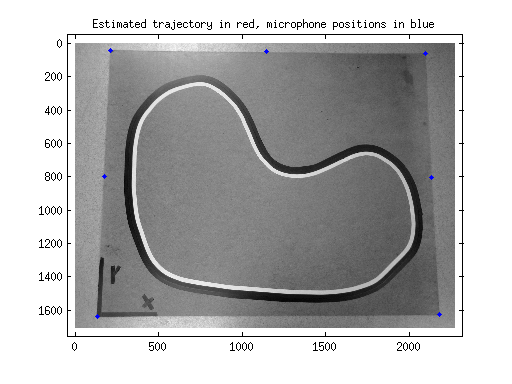
\includegraphics[scale=0.9]{microphone_pos_good.png}
\end{figure}

\begin{figure}[!h]
  \caption{Microphone setup two.}
  \label{bad_setup}
  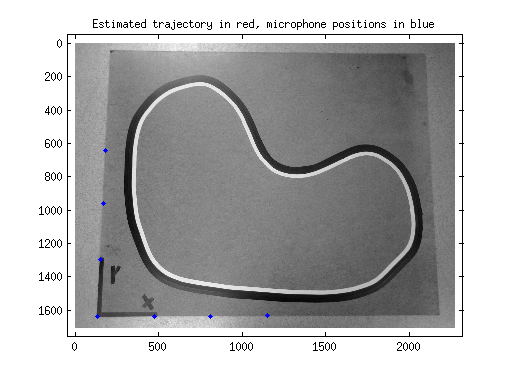
\includegraphics[scale=0.9]{microphone_pos_bad.png}
\end{figure}

\newpage
\chapter{Tasks}
\label{Tasks}

\newpage
\section{Calibration}
\label{Calibration}

\newpage
\section{Sensor modeling}
\label{Sensor modeling}

\newpage
\section{Experiments}
\label{Experiments}

\newpage
\section{Configuration analysis}
\label{Configuration analysis}

\newpage
\section{Localisation}
\label{Localisationg}

\newpage
\section{Tracking}
\label{Tracking}

\newpage
\section{Sensitivity analysis}
\label{Sensitivity analysis}

\end{document}



%%% Local Variables: 
%%% TeX-PDF-mode: t 
%%% TeX-master: "rapport"
%%% End: 

